% Generated from the public primitive catalog. Original Atlas drawing; Apache-2.0.
% Target: x448; view: overview
\documentclass[border=9pt]{standalone}
% Original Atlas figure theme. Apache-2.0; see the repository LICENSE.
\usepackage[T1]{fontenc}
\usepackage{lmodern}
\usepackage{amsmath,amssymb}
\usepackage{tikz}
\usetikzlibrary{arrows.meta,positioning,calc,fit,backgrounds,decorations.pathreplacing,matrix}
\definecolor{atlasInk}{HTML}{172235}
\definecolor{atlasTeal}{HTML}{0D7B7D}
\definecolor{atlasMuted}{HTML}{637278}
\definecolor{atlasFill}{HTML}{EAF4F2}
\definecolor{atlasLine}{HTML}{B6C8C7}
\tikzset{
  every picture/.style={line width=.65pt,draw=atlasInk,>=Latex},
  every node/.style={text=atlasInk,font=\sffamily\small},
  box/.style={draw,rounded corners=1.5pt,minimum height=.9cm,minimum width=1.6cm,align=center,inner sep=6pt,fill=white},
  accent/.style={box,draw=atlasTeal,fill=atlasFill},
  wire/.style={->,line width=.7pt},
  keywire/.style={wire,draw=atlasTeal,dashed},
  xor/.style={draw,circle,fill=white,inner sep=0pt,minimum size=.38cm},
  add/.style={draw,rectangle,fill=white,inner sep=0pt,minimum size=.38cm},
  note/.style={font=\sffamily\scriptsize,text=atlasMuted,align=center},
  phase/.style={font=\sffamily\small\bfseries,text=atlasTeal},
  group/.style={draw=atlasLine,dashed,rounded corners=2pt,inner sep=8pt}
}
\newcommand{\rotl}{\mathbin{\lll}}
\newcommand{\rotr}{\mathbin{\ggg}}
\newcommand{\kx}{\operatorname{Keccak}\!\text{-}\!f[1600]}

\newcommand{\AtlasModulusBits}{b}
\newcommand{\AtlasFieldBits}{448}
\newcommand{\AtlasHash}{\textsf{H}}
\newcommand{\AtlasCurve}{\textsf{curve}}
\newcommand{\AtlasDhGroup}{\textsf{X448}}
\newcommand{\AtlasDhPublicA}{\operatorname{XDH}(a,u_0)}
\newcommand{\AtlasDhPublicB}{\operatorname{XDH}(b,u_0)}
\newcommand{\AtlasDhSharedA}{\operatorname{XDH}(a,B)}
\newcommand{\AtlasDhSharedB}{\operatorname{XDH}(b,A)}
\newcommand{\AtlasSaltBytes}{s}
\newcommand{\AtlasSharedBits}{klen}
\newcommand{\AtlasPublicKeyBytes}{56}
\newcommand{\AtlasSecretKeyBytes}{|sk|}
\newcommand{\AtlasCiphertextBytes}{|c|}
\newcommand{\AtlasSignatureBytes}{|\sigma|}
\newcommand{\AtlasModuleRank}{k}
\newcommand{\AtlasMatrixRows}{k}
\newcommand{\AtlasMatrixColumns}{\ell}
\newcommand{\AtlasHypertreeHeight}{h}
\newcommand{\AtlasHypertreeLayers}{d}
\newcommand{\AtlasForsHeight}{a}
\newcommand{\AtlasForsTrees}{k}
\newcommand{\AtlasHashBytes}{n}
\newcommand{\AtlasHashFamily}{\textsf{SHA2 / SHAKE}}
\begin{document}
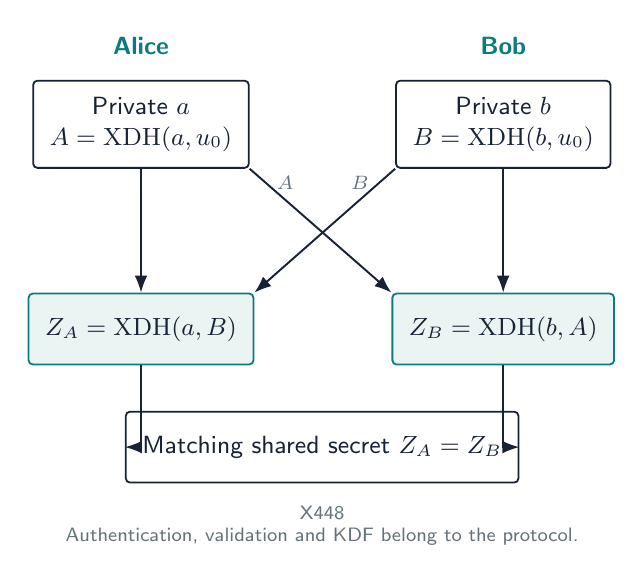
\begin{tikzpicture}
  \node[phase] at (0,0) {Alice}; \node[phase] at (4.6,0) {Bob};
  \node[box] (a) at (0,-1) {Private $a$\\$A=\AtlasDhPublicA$};
  \node[box] (b) at (4.6,-1) {Private $b$\\$B=\AtlasDhPublicB$};
  \node[accent] (sa) at (0,-3.6) {$Z_A=\AtlasDhSharedA$};
  \node[accent] (sb) at (4.6,-3.6) {$Z_B=\AtlasDhSharedB$};
  \draw[wire] (a) -- (sa); \draw[wire] (b) -- (sb);
  \draw[wire] (a.south east) -- node[pos=.25,above,note] {$A$} (sb.north west);
  \draw[wire] (b.south west) -- node[pos=.25,above,note] {$B$} (sa.north east);
  \node[box] (shared) at (2.3,-5.1) {Matching shared secret $Z_A=Z_B$};
  \draw[wire] (sa.south) |- (shared.west); \draw[wire] (sb.south) |- (shared.east);
  \node[note,text width=6.8cm] at (2.3,-6.1) {$\AtlasDhGroup$\\Authentication, validation and KDF belong to the protocol.};
\end{tikzpicture}

\end{document}
